% CVPR 2025 Paper Template; see https://github.com/cvpr-org/author-kit

\documentclass[10pt,twocolumn,letterpaper]{article}

%%%%%%%%% PAPER TYPE  - PLEASE UPDATE FOR FINAL VERSION
% \usepackage{cvpr}              % To produce the CAMERA-READY version
% \usepackage[review]{cvpr}      % To produce the REVIEW version
\usepackage[pagenumbers]{cvpr} % To force page numbers, e.g. for an arXiv version

% Import additional packages in the preamble file, before hyperref
%
% --- inline annotations
%
\newcommand{\red}[1]{{\color{red}#1}}
\newcommand{\todo}[1]{{\color{red}#1}}
\newcommand{\TODO}[1]{\textbf{\color{red}[TODO: #1]}}
% --- disable by uncommenting  
% \renewcommand{\TODO}[1]{}
% \renewcommand{\todo}[1]{#1}



% It is strongly recommended to use hyperref, especially for the review version.
% hyperref with option pagebackref eases the reviewers' job.
% Please disable hyperref *only* if you encounter grave issues, 
% e.g. with the file validation for the camera-ready version.
%
% If you comment hyperref and then uncomment it, you should delete *.aux before re-running LaTeX.
% (Or just hit 'q' on the first LaTeX run, let it finish, and you should be clear).
\definecolor{cvprblue}{rgb}{0.21,0.49,0.74}
\usepackage[pagebackref,breaklinks,colorlinks,allcolors=cvprblue]{hyperref}

%%%%%%%%% PAPER ID  - PLEASE UPDATE
\def\paperID{*****} % *** Enter the Paper ID here
\def\confName{CVPR}
\def\confYear{2025}

%%%%%%%%% TITLE - PLEASE UPDATE
\title{SAM-IAM: Segmenting Arbitrary Motion for Image Applications Model}
%%%%%%%%% AUTHORS - PLEASE UPDATE
\author{Dominic Chui$^{\dagger}$\\
Brown University
\and Hancheng Lin$^{\dagger}$\\
Brown University
\and Gabrielle Shieh$^{\dagger}$\\
Brown University
\and Brian Xu$^{\dagger}$\\
Brown University
% For a paper whose authors are all at the same institution,
% omit the following lines up until the closing ``}''.
% Additional authors and addresses can be added with ``\and'',
% just like the second author.
% To save space, use either the email address or home page, not both
}

\begin{document}
\twocolumn[{%
            \renewcommand\twocolumn[1][]{#1}%
            \maketitle
            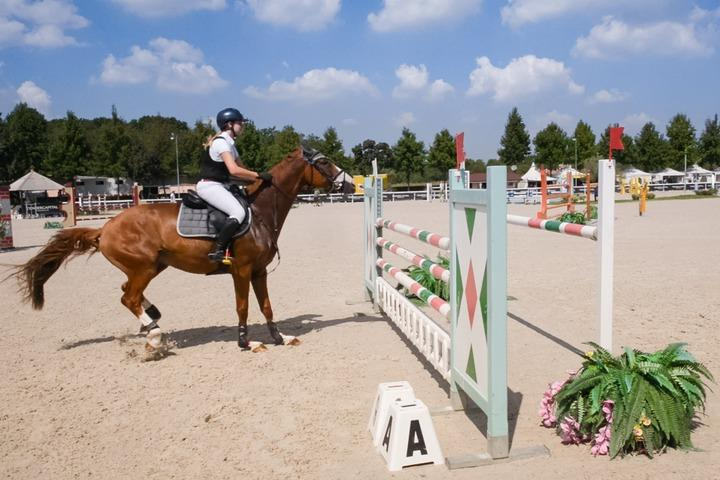
\includegraphics[width=.32\linewidth]{media/horse/ii.jpg}
            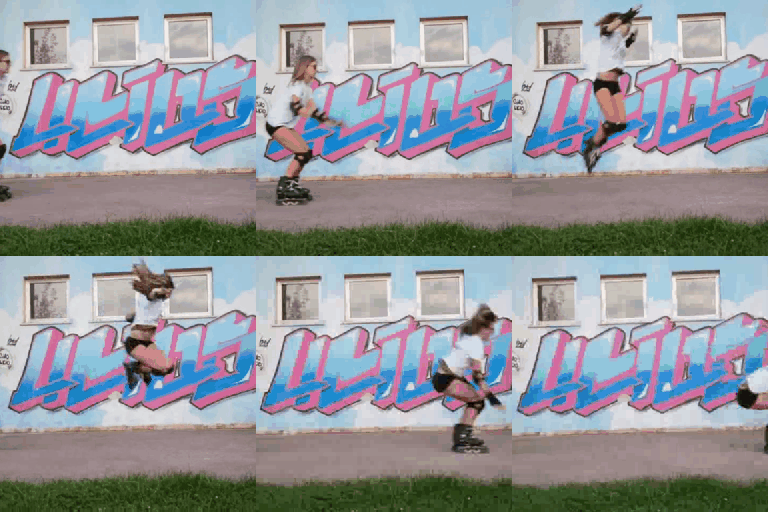
\includegraphics[width=.32\linewidth]{media/horse/dv.png}
            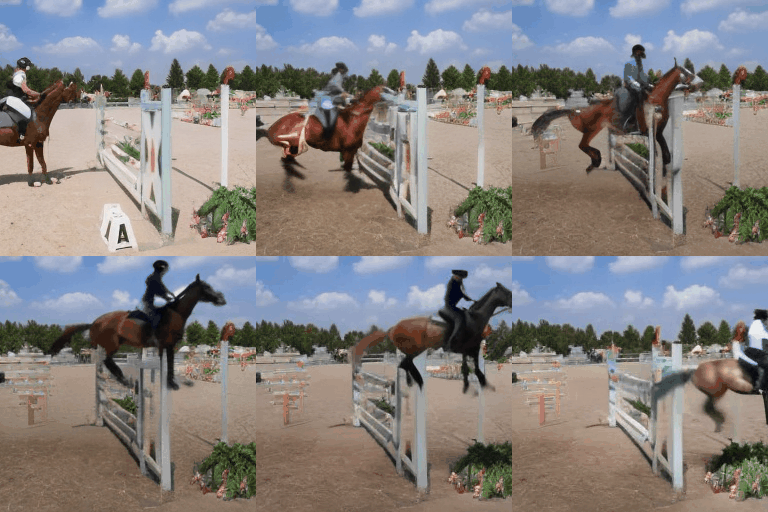
\includegraphics[width=.32\linewidth]{media/horse/ours.png}
            % \vspace{-2em}
            \captionof{figure}{Example output from our method.\vspace{1em}}
            \label{fig:teaser}
        }]
\begin{abstract}
    We present a novel modular video synthesis model for transfering the rigid motion from a driving video to a single image. SAM-IAM generates a new video by combining the subject of the input image and the motion of the input video. In constrast with diffusion models that are text, image, and even video conditioned, this offers an alternative generative approach with much creative potential. By first segmenting the driving video, the motion of the selected subject is isolated and approximated using tracking bounding boxes that can then be iteratively applied to the segmented subject of the input image. The stitching together and conversion of the segmentation masks is performed with an off-the-shelf diffusion model to generate temporally and spatially coherent videos. SAM-IAM shows great potential in generating realistic video results in a modular pipeline whose individual components can be iteratively improved upon.
        {\let\thefootnote\relax\footnote{{$^{\dagger}$Equal contribution}}}
\end{abstract}
\section{Introduction}
\label{sec:intro}

Please follow the steps outlined below when submitting your manuscript to the IEEE Computer Society Press.
This style guide now has several important modifications (for example, you are no longer warned against the use of sticky tape to attach your artwork to the paper), so all authors should read this new version.

%-------------------------------------------------------------------------
\subsection{Language}

All manuscripts must be in English.

\subsection{Dual submission}

Please refer to the author guidelines on the \confName\ \confYear\ web page for a
discussion of the policy on dual submissions.

\subsection{Paper length}
Papers, excluding the references section, must be no longer than eight pages in length.
The references section will not be included in the page count, and there is no limit on the length of the references section.
For example, a paper of eight pages with two pages of references would have a total length of 10 pages.
{\bf There will be no extra page charges for \confName\ \confYear.}

Overlength papers will simply not be reviewed.
This includes papers where the margins and formatting are deemed to have been significantly altered from those laid down by this style guide.
Note that this \LaTeX\ guide already sets figure captions and references in a smaller font.
The reason such papers will not be reviewed is that there is no provision for supervised revisions of manuscripts.
The reviewing process cannot determine the suitability of the paper for presentation in eight pages if it is reviewed in eleven.

%-------------------------------------------------------------------------
\subsection{The ruler}
The \LaTeX\ style defines a printed ruler which should be present in the version submitted for review.
The ruler is provided in order that reviewers may comment on particular lines in the paper without circumlocution.
If you are preparing a document using a non-\LaTeX\ document preparation system, please arrange for an equivalent ruler to appear on the final output pages.
The presence or absence of the ruler should not change the appearance of any other content on the page.
The camera-ready copy should not contain a ruler.
(\LaTeX\ users may use options of \texttt{cvpr.sty} to switch between different versions.)

Reviewers:
note that the ruler measurements do not align well with lines in the paper --- this turns out to be very difficult to do well when the paper contains many figures and equations, and, when done, looks ugly.
Just use fractional references (\eg, this line is $087.5$), although in most cases one would expect that the approximate location will be adequate.


\subsection{Paper ID}
Make sure that the Paper ID from the submission system is visible in the version submitted for review (replacing the ``*****'' you see in this document).
If you are using the \LaTeX\ template, \textbf{make sure to update paper ID in the appropriate place in the tex file}.


\subsection{Mathematics}

Please number all of your sections and displayed equations as in these examples:
\begin{equation}
  E = m\cdot c^2
  \label{eq:important}
\end{equation}
and
\begin{equation}
  v = a\cdot t.
  \label{eq:also-important}
\end{equation}
It is important for readers to be able to refer to any particular equation.
Just because you did not refer to it in the text does not mean some future reader might not need to refer to it.
It is cumbersome to have to use circumlocutions like ``the equation second from the top of page 3 column 1''.
(Note that the ruler will not be present in the final copy, so is not an alternative to equation numbers).
All authors will benefit from reading Mermin's description of how to write mathematics:
\url{http://www.pamitc.org/documents/mermin.pdf}.

\subsection{Blind review}

Many authors misunderstand the concept of anonymizing for blind review.
Blind review does not mean that one must remove citations to one's own work---in fact it is often impossible to review a paper unless the previous citations are known and available.

Blind review means that you do not use the words ``my'' or ``our'' when citing previous work.
That is all.
(But see below for tech reports.)

Saying ``this builds on the work of Lucy Smith [1]'' does not say that you are Lucy Smith;
it says that you are building on her work.
If you are Smith and Jones, do not say ``as we show in [7]'', say ``as Smith and Jones show in [7]'' and at the end of the paper, include reference 7 as you would any other cited work.

An example of a bad paper just asking to be rejected:
\begin{quote}
\begin{center}
    An analysis of the frobnicatable foo filter.
\end{center}

   In this paper we present a performance analysis of our previous paper [1], and show it to be inferior to all previously known methods.
   Why the previous paper was accepted without this analysis is beyond me.

   [1] Removed for blind review
\end{quote}


An example of an acceptable paper:
\begin{quote}
\begin{center}
     An analysis of the frobnicatable foo filter.
\end{center}

   In this paper we present a performance analysis of the  paper of Smith \etal [1], and show it to be inferior to all previously known methods.
   Why the previous paper was accepted without this analysis is beyond me.

   [1] Smith, L and Jones, C. ``The frobnicatable foo filter, a fundamental contribution to human knowledge''. Nature 381(12), 1-213.
\end{quote}

If you are making a submission to another conference at the same time, which covers similar or overlapping material, you may need to refer to that submission in order to explain the differences, just as you would if you had previously published related work.
In such cases, include the anonymized parallel submission~\cite{Authors14} as supplemental material and cite it as
\begin{quote}
[1] Authors. ``The frobnicatable foo filter'', F\&G 2014 Submission ID 324, Supplied as supplemental material {\tt fg324.pdf}.
\end{quote}

Finally, you may feel you need to tell the reader that more details can be found elsewhere, and refer them to a technical report.
For conference submissions, the paper must stand on its own, and not {\em require} the reviewer to go to a tech report for further details.
Thus, you may say in the body of the paper ``further details may be found in~\cite{Authors14b}''.
Then submit the tech report as supplemental material.
Again, you may not assume the reviewers will read this material.

Sometimes your paper is about a problem which you tested using a tool that is widely known to be restricted to a single institution.
For example, let's say it's 1969, you have solved a key problem on the Apollo lander, and you believe that the 1970 audience would like to hear about your
solution.
The work is a development of your celebrated 1968 paper entitled ``Zero-g frobnication: How being the only people in the world with access to the Apollo lander source code makes us a wow at parties'', by Zeus \etal.

You can handle this paper like any other.
Do not write ``We show how to improve our previous work [Anonymous, 1968].
This time we tested the algorithm on a lunar lander [name of lander removed for blind review]''.
That would be silly, and would immediately identify the authors.
Instead write the following:
\begin{quotation}
\noindent
   We describe a system for zero-g frobnication.
   This system is new because it handles the following cases:
   A, B.  Previous systems [Zeus et al. 1968] did not  handle case B properly.
   Ours handles it by including a foo term in the bar integral.

   ...

   The proposed system was integrated with the Apollo lunar lander, and went all the way to the moon, don't you know.
   It displayed the following behaviours, which show how well we solved cases A and B: ...
\end{quotation}
As you can see, the above text follows standard scientific convention, reads better than the first version, and does not explicitly name you as the authors.
A reviewer might think it likely that the new paper was written by Zeus \etal, but cannot make any decision based on that guess.
He or she would have to be sure that no other authors could have been contracted to solve problem B.
\medskip

\noindent
FAQ\medskip\\
{\bf Q:} Are acknowledgements OK?\\
{\bf A:} No.  Leave them for the final copy.\medskip\\
{\bf Q:} How do I cite my results reported in open challenges?
{\bf A:} To conform with the double-blind review policy, you can report results of other challenge participants together with your results in your paper.
For your results, however, you should not identify yourself and should not mention your participation in the challenge.
Instead present your results referring to the method proposed in your paper and draw conclusions based on the experimental comparison to other results.\medskip\\

\begin{figure}[t]
  \centering
  \fbox{\rule{0pt}{2in} \rule{0.9\linewidth}{0pt}}
   %\includegraphics[width=0.8\linewidth]{egfigure.eps}

   \caption{Example of caption.
   It is set in Roman so that mathematics (always set in Roman: $B \sin A = A \sin B$) may be included without an ugly clash.}
   \label{fig:onecol}
\end{figure}

\subsection{Miscellaneous}

\noindent
Compare the following:\\
\begin{tabular}{ll}
 \verb'$conf_a$' &  $conf_a$ \\
 \verb'$\mathit{conf}_a$' & $\mathit{conf}_a$
\end{tabular}\\
See The \TeX book, p165.

The space after \eg, meaning ``for example'', should not be a sentence-ending space.
So \eg is correct, {\em e.g.} is not.
The provided \verb'\eg' macro takes care of this.

When citing a multi-author paper, you may save space by using ``et alia'', shortened to ``\etal'' (not ``{\em et.\ al.}'' as ``{\em et}'' is a complete word).
If you use the \verb'\etal' macro provided, then you need not worry about double periods when used at the end of a sentence as in Alpher \etal.
However, use it only when there are three or more authors.
Thus, the following is correct:
   ``Frobnication has been trendy lately.
   It was introduced by Alpher~\cite{Alpher02}, and subsequently developed by
   Alpher and Fotheringham-Smythe~\cite{Alpher03}, and Alpher \etal~\cite{Alpher04}.''

This is incorrect: ``... subsequently developed by Alpher \etal~\cite{Alpher03} ...'' because reference~\cite{Alpher03} has just two authors.

\begin{figure*}
  \centering
  \begin{subfigure}{0.68\linewidth}
    \fbox{\rule{0pt}{2in} \rule{.9\linewidth}{0pt}}
    \caption{An example of a subfigure.}
    \label{fig:short-a}
  \end{subfigure}
  \hfill
  \begin{subfigure}{0.28\linewidth}
    \fbox{\rule{0pt}{2in} \rule{.9\linewidth}{0pt}}
    \caption{Another example of a subfigure.}
    \label{fig:short-b}
  \end{subfigure}
  \caption{Example of a short caption, which should be centered.}
  \label{fig:short}
\end{figure*}

\section{Related works}
\label{sec:related_work}

Much related work in video synthesis have tended to fall into either category of image-to-video methods or video diffusion models.

%-------------------------------------------------------------------------
\subsection{Image-to-Video Methods}

Image-to-video methods exist in two flavors: diffusion and non-diffusion based. Periodic patterns have been manipulated to generate seamlessly animated \emph{endless loops} \cite{Halperin_2021} in a non-machine learning approach, while neural network architecture has been employed in a \emph{conditional invertible neural network (cINN)} architecture \cite{dorkenwald2021stochasticimagetovideosynthesisusing}. 

Diffusion based image-to-video methods rely on the remarkable performance of diffusion models in image synthesis by extending the existing text-to-video models with temporal-consistency attention layers for image-to-video synthesis and larger training datasets \cite{blattmann2023stablevideodiffusionscaling}. This approach has seen applications in character animation \cite{hu2024animateanyoneconsistentcontrollable} and fashion posing \cite{52750}. ControlNet \cite{zhang2023addingconditionalcontroltexttoimage} style approaches extended to video have also been succesfully built \cite{zhang2023controlvideotrainingfreecontrollabletexttovideo}.


%-------------------------------------------------------------------------
\subsection{Video Diffusion}

With the success of text-to-image and image-to-video models, diffusion models have been successfully developed for training directly on videos themselves in the video-to-video mode. The major obstacle of temporal consistency and coherence has been tackled in a variety of different ways, typically relying on a pretrained diffusion model supplemented with carefully augmented attention layers and conditioning \cite{melnik2024videodiffusionmodelssurvey}. Controllable video synthesis that allows for user guidance in textual, spatial, and temporal forms have been explored by using motion vectors and spatio-temporal condition encoders \cite{wang2023videocomposercompositionalvideosynthesis}, propagating and injecting condition features through condition adapters \cite{wang2024easycontroltransfercontrolnetvideo}, and explicit motion modeling \cite{shi2024motioni2vconsistentcontrollableimagetovideo}.

\subsection{Conditioning Object Motion}

Conditioning object motion can be viewed as a form of spatio-temporal guidance in video generation. Diffusion-based video generative models supporting motion control can be categorized based on the specificity and type of input they use.

At one end of the spectrum, detailed spatial conditioning sequences are used as frame-by-frame guidance. These spatial constraints, in the form of optical flow \cite{ni2023conditional}, motion vector \cite{2023videocomposer}, pose \cite{feng2023dreamoving}, depth \cite{2023videocomposer, feng2023dreamoving}, and sketch outline \cite{2023videocomposer}, enable precise control over the generated video. Focusing on specific applications, specialized frameworks have been proposed to customize human videos \cite{feng2023dreamoving}. When applied to objects of a different kind, these methods often yield results akin to style transfers. The strong spatial constraint sequences used by these methods limits their capability in adaptively transferring motion properties between different object types.

On the opposite end, more abstract representations, such as motion flows represented by arrows \cite{yin2023dragnuwa, 2023videocomposer} and vectors \cite{2023videocomposer} or motion themes like ‘inflate,’ ‘squish,’ or ‘crumble’ \cite{Pikaffect}, are used as motion guidance. These methods offer greater generalization across various object classes while compromising on the control over specific motion details and relative frame positioning.

This paper proposes a modular video generation pipeline with a bounding-box driven motion transfer implementation. The method seeks to explore a midpoint in the spectrum of motion control, offering an alternative perspective and demonstrating its generative potential. The goal is to retain control over relative frame positions and overall motion from the driving video, rather than requiring detailed, instance-aligned spatial conditioning sequences. This approach aims to enable more flexible and realistic adaptations of motion characteristics in video generation.


\begin{figure}[t]
    \centering
    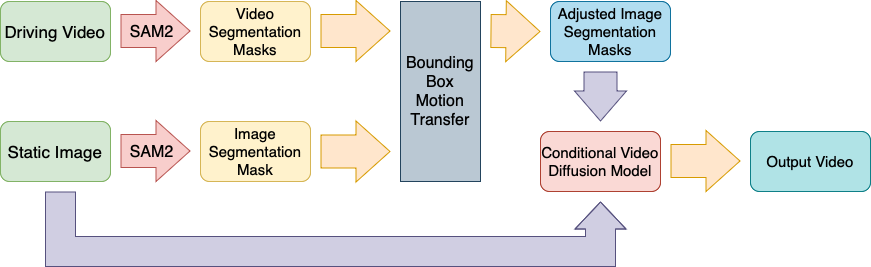
\includegraphics[width=1\linewidth]{media/method.png}
    % \vspace{-2em}
    \captionof{figure}{An overview of our pipeline.}
    \label{fig:method}
\end{figure}

\section{Method}

We provide an overview of our method in \cref{fig:method}. Our inputs are a video (also referred to as the "driving video") and a static image.
We apply an off-the-shelf image and video segmentation model\cite{ravi2024sam2} to obtain binary segmentation masks of the foreground object.
For the video, we obtain a segmentation mask for each frame, tracking the relative motion of the masked object.
We use a bounding box approach to calculate the change in position and scale for each frame in the video mask.
Given this per-frame deformation, we can sequentially modify the segmentation mask of the input image to replicate motion analogous to the driving video.
Finally, we use the motion-transferred video along with the original image as inputs for a conditional video diffusion model\cite{2023videocomposer}.

%-------------------------------------------------------------------------
\subsection{Image and Video Segmentation}

We use an off-the-shelf segmentation model\cite{ravi2024sam2} for both the image and the video.
Due to the importance of obtaining proper segmentation masks, we elect to involve the user during this step.
We present the user a GUI (see \cref{fig:ui}), allowing them to interactively select which foreground objects are segmented.

\begin{figure}[t]
    \centering
    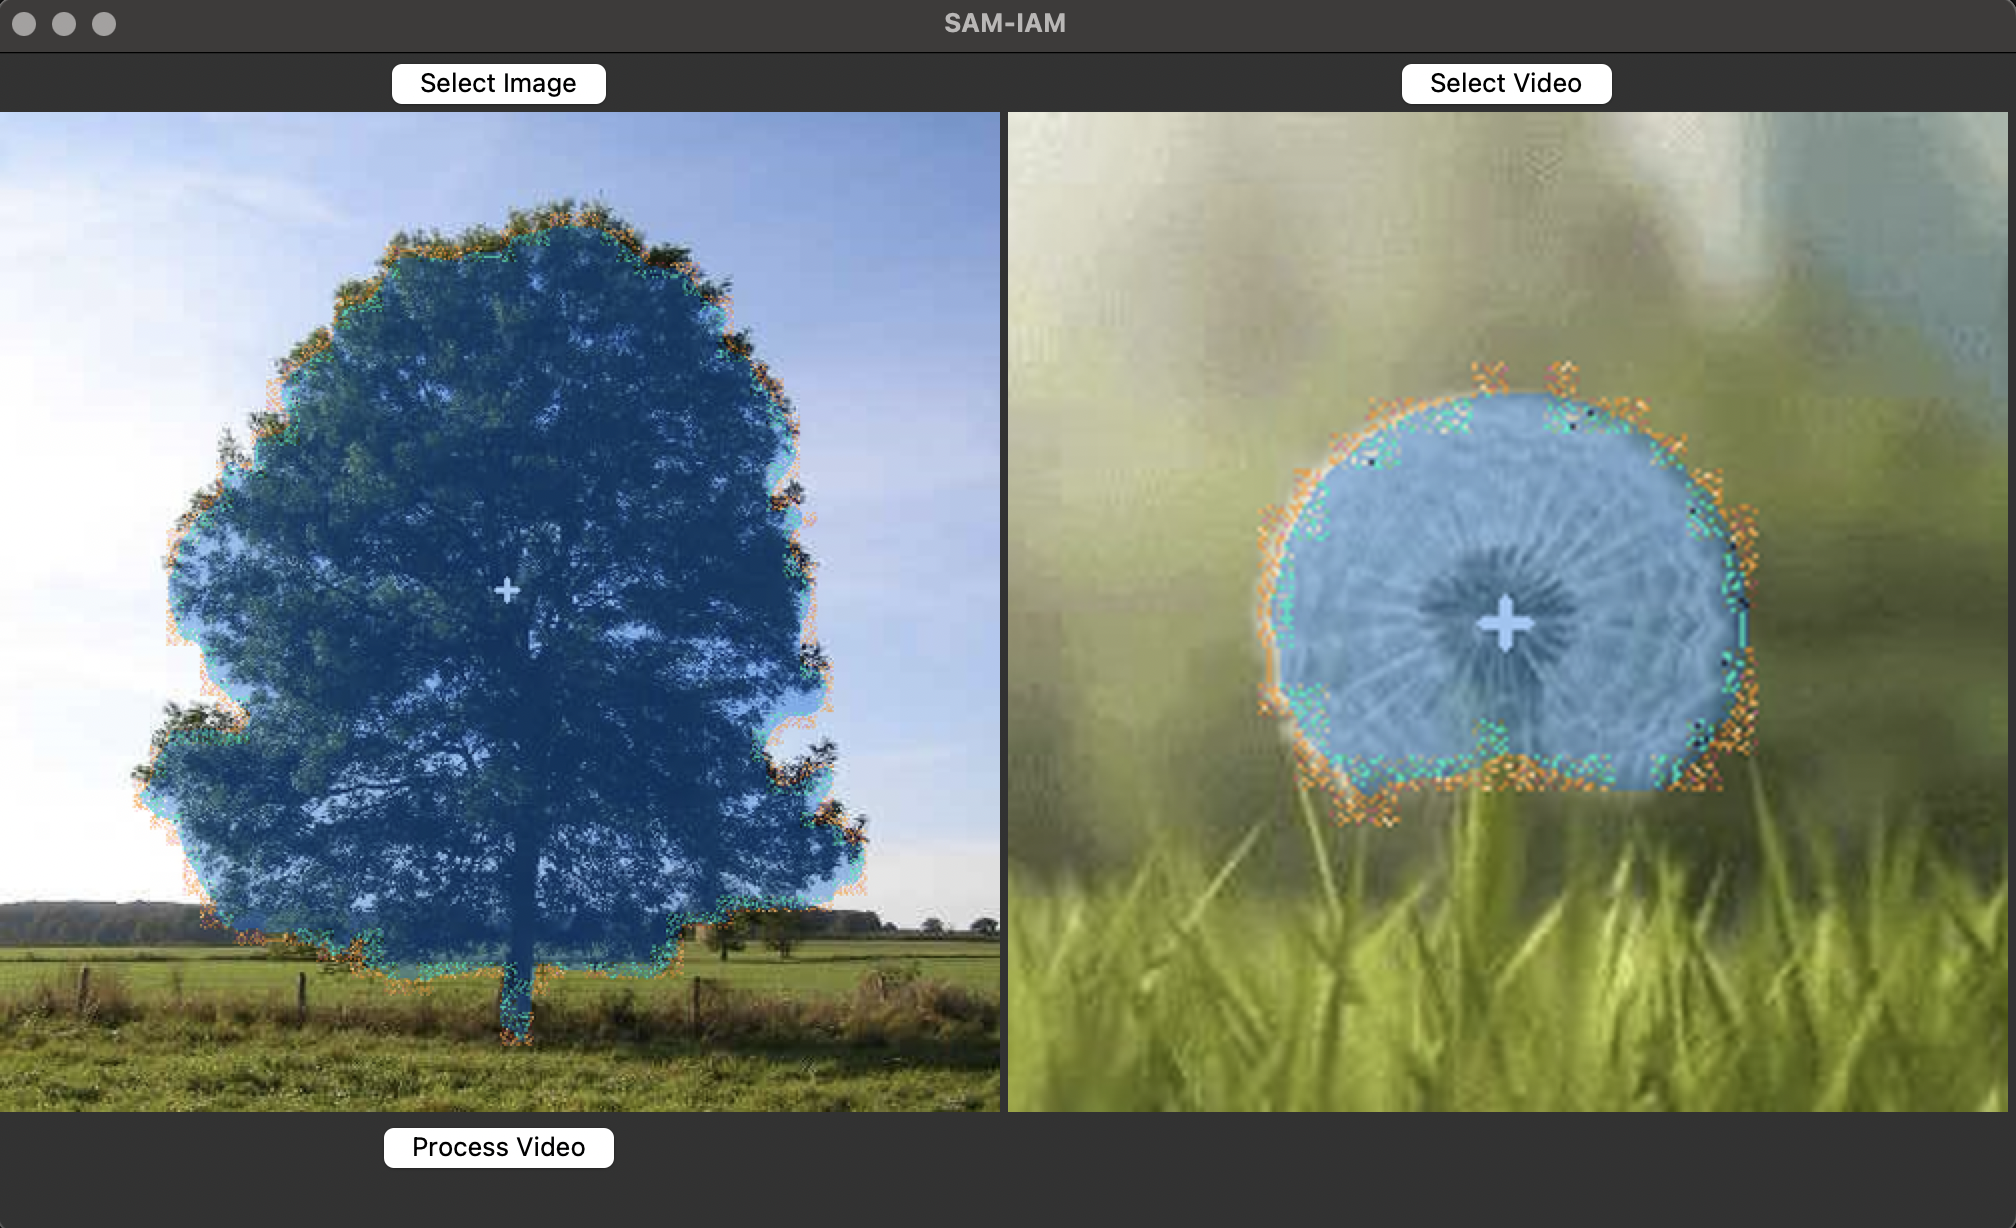
\includegraphics[width=1\linewidth]{media/ui.png}
    \caption{A screenshot of our segmentation UI.}
    \label{fig:ui}
\end{figure}

%-------------------------------------------------------------------------
\subsection{Bounding Box Motion Transfer}


Given a binary segmentation mask, it is trivial to draw a bounding box around it. We can obtain a rough estimate for the relative motion of a video by calculating the change in position and scale between each frame.
For each frame in the driving video, we obtain a translation \textit{t} and change in scale \textit{s} of its corresponding bounding box, relative to the first frame.
\begin{equation}
    \begin{gathered}
        t_{n} = (bbox_{vid_n}.x-bbox_{vid_0}.x, bbox_{vid_n}.y-bbox_{vid_0}.y) \\
        s_{n} = (\frac{bbox_{vid_n}.width}{bbox_{vid_0}.width},\frac{bbox_{vid_n}.height}{bbox_{vid_0}.height})
    \end{gathered}
    \label{eq:transformation}
\end{equation}

To preserve the direction of motion while accounting for possible differences in size, we introduce scaling factors \textit{x} and \textit{y}.
These scaling factors are equal to the height and width ratios of the bounding boxes for the input image and first frame of the driving video.
\begin{equation}
    \begin{gathered}
        x = \frac{bbox_{img}.width}{bbox_{vid}.width} \\ y = \frac{bbox_{img}.height}{bbox_{vid}.height}
    \end{gathered}
    \label{eq:scaling}
\end{equation}

We sequentially apply the adjusted set of translations and scales to the mask of the input image to obtain a target video \textit{V}, which we use as input for a conditional diffusion model\cite{2023videocomposer}.
\begin{equation}
    \begin{gathered}
        V_{n}.size = bbox_{img}.size*s_{n}*(x,y) \\
        V_{n}.pos = bbox_{img}.pos + t_{n}*(x,y) \\
        V_{n}.pos = V_{n}.pos - \frac{(V_{n}.size-bbox_{n}.size)}{2}
    \end{gathered}
\end{equation}

\section{Experiments}

We evaluated our method on several image-video pairs. For a baseline comparison, we used the same inputs on our off-the-shelf model to provide a fair comparison.
\section{Discussion}

\subsection{Results}
We demonstrate the performance of our approach against our baseline, VideoComposer, a controllable video diffusion model. In Table 1, we demonstrate our results through a side-by-side comparison with VideoComposer. As shown, the existing baseline fails to capture the intrinsics of the subject's change in motion, and even in some cases fails to comprehend the motion dynamics of the original driving video. We see in parachute example that SAM-IAM captures the shape of the parachute throughout the length of the projected motion, whereas VideoComposer suffers from shape deformation. Furthermore, the soccer ball example demonstrates the ability of SAM-IAM to comprehend more complex motions as the driving video illustrates a car traveling across the frame from right to left, with the addition of forward motion towards the camera in the beginning frames. However, VideoComposer fails to correctly capture the scale of the input image while adding additional artifacts to the resulting video.

In the equestrian example, we qualitatively compare SAM-IAM and VideoComposer on a driving video that exhibits human motion in the form of jumping. While VideoComposer adds artifacts to the foreground and background of the frame and incorrectly adds rotation to the target object's movement, SAM-IAM cleanly translates the movement of the jumping rollerblader to the horse in the same arcing motion.

In the case of occlusion, SAM-IAM achieves an accurate representation by adding another moving vehicle to obstruct the view of the car, analogous to the way the plant occludes the motorcycle in the driving video. In contrast, VideoComposer exhibits multiple colliding vehicles to its resulting video, demonstrating a lack of understanding of occlusion. 

\subsection{Method Limitations}

We initially decided on an autoencoder to understand the motion demonstrated in the driving video. The autoencoder is passed the input image and frames \textit{n} and \textit{n + 1} of the driving video, and creates a difference map from the video frames to pass into the encoder. The encoder outputs the latent code, which, with the input frame, would be passed into the decoder to reconstruct the predicted next image frame. However, after training and testing this model on the DAVIS dataset, we found that the autoencoder was greatly overfitting because transferring motion across different classes of object requires a deep understanding of their geometric properties and our frame-by-frame approach led to unstable and inconsistent motions. We theorize these shortcomings could be alleviated with a stronger dataset containing paired data for the type of ‘loose’ motion transfer we want and a loss function that captures the intricacies of the underlying motion rather than basic change in position across frames. 

Due to the modal nature of our pipeline, we were easily able to pivot and replace the autoencoder with the bounding box method outlined in our paper to track the motion in the driving video. 

\section{Conclusion}

qualitative review of results and how we can improve

Future research could focus on several aspects to enhance the versatility of video-driven motion control in video generation. Refining the granularity of segmentation in motion objects extracted from driving videos could improve the quality of motion guidance used to condition the output video in our pipeline. Additionally, integrating a feature extraction diffusion model \cite{luo2024diffusion} could provide a more semantic mapping of motion details between objects, thereby strengthening the adaptability of motion transfers.

Another direction could involve adopting more sophisticated generative models, such as Variational Autoencoders (VAEs) and diffusion models, for the motion extraction and transfer phases. This approach would require collecting extensive paired data and might be susceptible to inherent biases, such as viewpoint bias, which needs to be considered.

{
    \small
    \bibliographystyle{ieeenat_fullname}
    \bibliography{main}
}

% WARNING: do not forget to delete the supplementary pages from your submission 
% \clearpage
\setcounter{page}{1}
\maketitlesupplementary


\section{Rationale}
\label{sec:rationale}
% 
Having the supplementary compiled together with the main paper means that:
% 
\begin{itemize}
\item The supplementary can back-reference sections of the main paper, for example, we can refer to \cref{sec:intro};
\item The main paper can forward reference sub-sections within the supplementary explicitly (e.g. referring to a particular experiment); 
\item When submitted to arXiv, the supplementary will already included at the end of the paper.
\end{itemize}
% 
To split the supplementary pages from the main paper, you can use \href{https://support.apple.com/en-ca/guide/preview/prvw11793/mac#:~:text=Delete%20a%20page%20from%20a,or%20choose%20Edit%20%3E%20Delete).}{Preview (on macOS)}, \href{https://www.adobe.com/acrobat/how-to/delete-pages-from-pdf.html#:~:text=Choose%20%E2%80%9CTools%E2%80%9D%20%3E%20%E2%80%9COrganize,or%20pages%20from%20the%20file.}{Adobe Acrobat} (on all OSs), as well as \href{https://superuser.com/questions/517986/is-it-possible-to-delete-some-pages-of-a-pdf-document}{command line tools}.

\end{document}
